\begin{flushright} {\tiny {\color{gray} basis\_Q1\_2D.tex}} \end{flushright}
%~~~~~~~~~~~~~~~~~~~~~~~~~~~~~~~~~~~~~~~~~~~~~~~~~~~~~~~~~~~~~~~~~~~~~~~~~~~~~~~~~~~~~~~~~~~~~~~~~~

In this section, we consider for simplicity an element which is a square defined 
by $-1<r<1$, $-1<s<1$ in the Cartesian coordinates system $(r,s)$\footnote{There is a 
reason to choose $r$ and $s$ as coordinates and not $x$ and $y$ as we will see later.}:

\begin{flushright} {\tiny {\color{gray} (tikz\_q12d.tex)}} \end{flushright}
%~~~~~~~~~~~~~~~~~~~~~~~~~~~~~~~~~~~~~~~~~~~~~~~~~~~~~~~~~~~~~~~~~~~~~~~~~~~~~~~~~~~~~~~~~~~~~~~~~~

\begin{center}
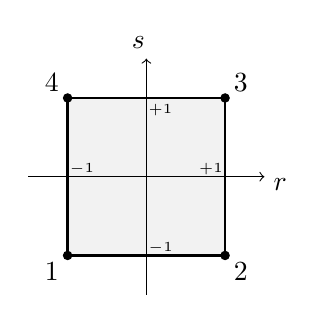
\begin{tikzpicture}
%\draw[step=0.5cm,gray,very thin] (0,0) grid (4,4); 
\draw[fill=gray!10,gray!10](1,1) rectangle (3,3);
\draw[thick] (1,1)--(3,1)--(3,3)--(1,3)--cycle;
\draw [->] (0.5,2) -- (3.5,2);
\draw [->] (2,0.5) -- (2,3.5);
\node[] at (3.7,1.9) {$r$};
\node[] at (1.9,3.7) {$s$};
\draw[black,fill=black] (1,1)   circle (1.5pt);
\draw[black,fill=black] (3,1)   circle (1.5pt);
\draw[black,fill=black] (3,3)   circle (1.5pt);
\draw[black,fill=black] (1,3)   circle (1.5pt);
\node[] at (0.8,0.8) {$1$};
\node[] at (0.8,3.2) {$4$};
\node[] at (3.2,0.8) {$2$};
\node[] at (3.2,3.2) {$3$};
\node[] at (1.18,2.1) {\tiny $-1$};
\node[] at (2.82,2.1) {\tiny $+1$};
\node[] at (2.18,1.1) {\tiny $-1$};
\node[] at (2.18,2.85) {\tiny $+1$};
\end{tikzpicture}
\end{center}



Note the counter-clockwise numbering\footnote{Note that in many of the python codes which 
are part of this project the numbering starts at 0.}.
This element is commonly called the reference element. How we go from the $(x,y)$ coordinate system 
to the $(r,s)$ once and vice versa will be dealt with later on.
The basis functions in the above reference element in the reduced 
coordinates system $(r,s)$ are given by:

\begin{mdframed}[backgroundcolor=blue!5]
\begin{eqnarray}
\bN_1(r,s)&=&0.25(1-r)(1-s) \nonumber\\
\bN_2(r,s)&=&0.25(1+r)(1-s) \nonumber\\
\bN_3(r,s)&=&0.25(1+r)(1+s) \nonumber\\
\bN_4(r,s)&=&0.25(1-r)(1+s) 
\end{eqnarray}
\end{mdframed}
These basis functions are the product of the linear basis functions of Section~\ref{sec:bf1}
in the $r$ direction and the $s$ direction.

\begin{center}
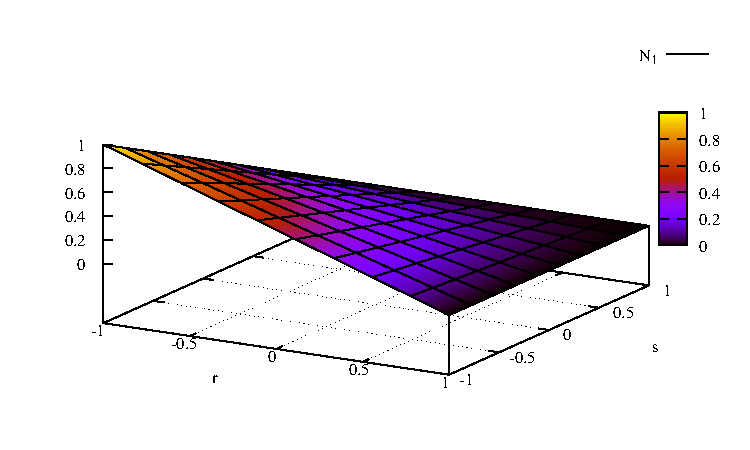
\includegraphics[width=4cm]{images/basis_Q1_2D/N1}
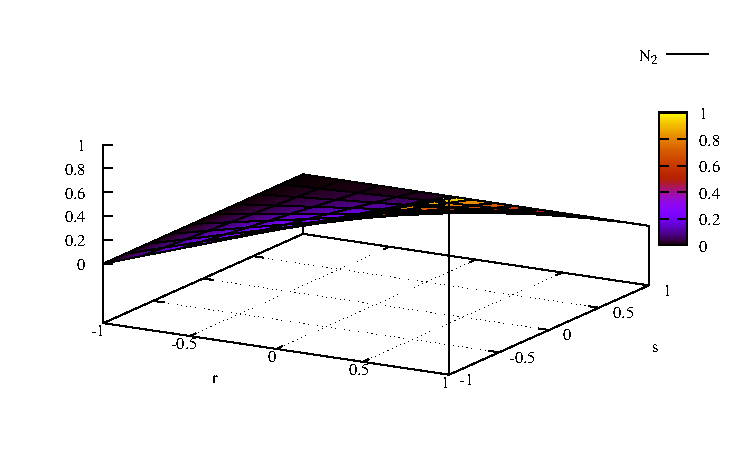
\includegraphics[width=4cm]{images/basis_Q1_2D/N2}
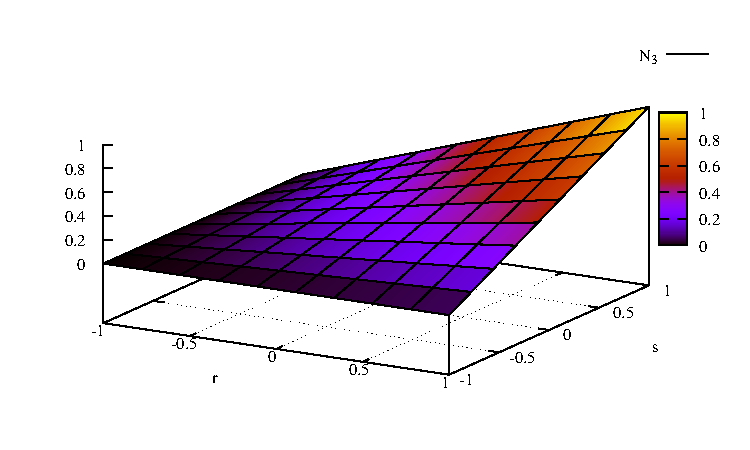
\includegraphics[width=4cm]{images/basis_Q1_2D/N3}
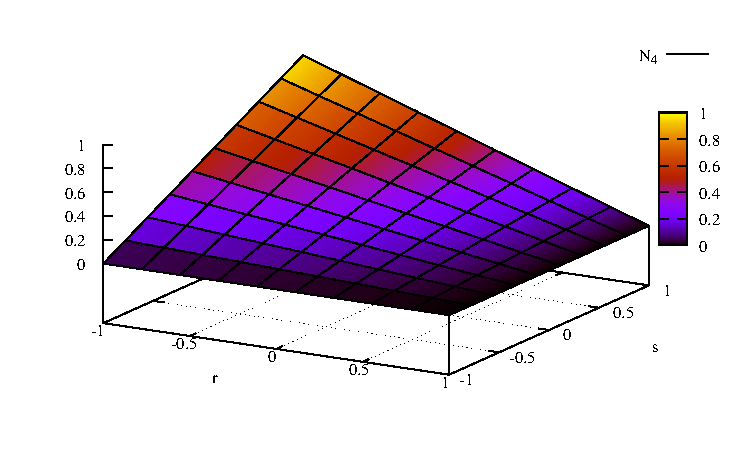
\includegraphics[width=4cm]{images/basis_Q1_2D/N4}\\
{\captionfont Surface representation of the basis functions on the reference element.\\
{\color{gray} in images/basis\_Q1\_2D/ }}
\end{center}


The partial derivatives of these functions with respect to $r$ ans $s$ automatically follow:

\begin{mdframed}[backgroundcolor=blue!5]
\begin{align}
\frac{\partial \bN_1}{\partial r}(r,s)&= - 0.25(1-s) &
\frac{\partial \bN_1}{\partial s}(r,s)&= - 0.25(1-r) \nonumber\\
\frac{\partial \bN_2}{\partial r}(r,s)&= + 0.25(1-s) &
\frac{\partial \bN_2}{\partial s}(r,s)&= - 0.25(1+r) \nonumber\\
\frac{\partial \bN_3}{\partial r}(r,s)&= + 0.25(1+s) &
\frac{\partial \bN_3}{\partial s}(r,s)&= + 0.25(1+r) \nonumber\\
\frac{\partial \bN_4}{\partial r}(r,s)&= - 0.25(1+s) &
\frac{\partial \bN_4}{\partial s}(r,s)&= + 0.25(1-r) \nonumber
\end{align}
\end{mdframed}

Let us go back to Eq.~\eqref{bf01} and let us assume that the 
function $v(r,s)=C$ so that $v_i=C$ for $i=1,2,3,4$. 
It then follows that 
\[
v^h(r,s) = \sum_{i=1}^4 \bN_i(r,s)\;  v_i 
=C \sum_{i=1}^4 \bN_i(r,s)
=C [
\bN_1(r,s)
+\bN_2(r,s)
+\bN_3(r,s)
+\bN_4(r,s)]=C
\]
This is a very important property: if the $v$ function used to 
assign values at the vertices is constant, then 
the value of $v^h$ {\it anywhere} in the element is exactly $C$.
If we now turn to the derivatives of $v$ with respect to $r$ and $s$:
\[
\frac{\partial {v}^h}{\partial r}(r,s) 
= \sum_{i=1}^4 \frac{\partial \bN_i}{\partial r}(r,s)\;  v_i 
= C \sum_{i=1}^4 \frac{\partial \bN_i}{\partial r}(r,s) 
= C \left[ - 0.25(1-s)  + 0.25(1-s)  + 0.25(1+s)  - 0.25(1+s) \right] = 0 
\]

\[
\frac{\partial v^h}{\partial s}(r,s) 
= \sum_{i=1}^4 \frac{\partial \bN_i}{\partial s}(r,s)\;  v_i 
= C \sum_{i=1}^4 \frac{\partial \bN_i}{\partial s}(r,s) 
= C \left[ - 0.25(1-r) - 0.25(1+r) + 0.25(1+r) + 0.25(1-r) \right] = 0 
\]
We reassuringly find that the derivative of a constant field anywhere in the element is exactly zero.

If we now choose $v(r,s)=ar+bs$ with $a$ and $b$ two constant scalars, we find:
\begin{eqnarray}
v^h(r,s) 
&=& \sum_{i=1}^4 \bN_i(r,s)\;  v_i  \nn\\
&=& \sum_{i=1}^4 \bN_i(r,s) (ar_i+bs_i) \nn\\
&=& a \sum_{i=1}^4 \bN_i(r,s) r_i + b \sum_{i=1}^4 \bN_i(r,s) s_i \nn\\
&=& a \left[ 
 \frac14(1-r)(1-s)(-1)
+\frac14(1+r)(1-s)(+1)
+\frac14(1+r)(1+s)(+1)
+\frac14(1-r)(1+s)(-1) \right]  \nonumber\\
&+& b  
\left[ 
 \frac14(1-r)(1-s)(-1)
+\frac14(1+r)(1-s)(-1)
+\frac14(1+r)(1+s)(+1)
+\frac14(1-r)(1+s)(+1) \right]  \nonumber\\
&=& \frac{a}{4} \left[ 
-(1-r)(1-s)
+(1+r)(1-s)
+(1+r)(1+s)
-(1-r)(1+s) \right]  \nonumber\\
&+& \frac{b}{4}
\left[ 
-(1-r)(1-s)
-(1+r)(1-s)
+(1+r)(1+s)
+(1-r)(1+s) 
\right]  \nonumber\\
&=& ar+bs
\end{eqnarray}
This set of bilinear basis functions is therefore capable of exactly representing a bilinear field.
The derivatives are:
\begin{eqnarray}
\frac{\partial v^h}{\partial r}(r,s) 
&=& \sum_{i=1}^4 \frac{\partial \bN_i}{\partial r}(r,s)\;  v_i  \nn\\
&=& a \sum_{i=1}^4 \frac{\partial \bN_i}{\partial r}(r,s) r_i 
+ b \sum_{i=1}^4 \frac{\partial \bN_i}{\partial r}(r,s) s_i \nn\\
&=& a \left[
- \frac14(1-s)(-1) 
+ \frac14(1-s)(+1) 
+ \frac14(1+s)(+1) 
- \frac14(1+s)(-1) 
\right] \nonumber\\
&+&b \left[
- \frac14(1-s)(-1) 
+ \frac14(1-s)(-1) 
+ \frac14(1+s)(+1) 
- \frac14(1+s)(+1) 
\right] \nonumber\\
&=& \frac{a}{4} \left[
 (1-s)
+ (1-s)
+ (1+s)
+ (1+s)
\right] \nonumber\\
&+&\frac{b}{4} \left[
 (1-s)
- (1-s)
+ (1+s)
- (1+s)
\right] \nonumber\\
&=& a 
\end{eqnarray}
Here again, we find that the derivative of the bilinear field inside the element is exact: 
$\frac{\partial v^h}{\partial r} = \frac{\partial v}{\partial r}$.

However, following the same methodology as above, one can easily prove 
that this is no more true for polynomials of degree strictly higher than 1. 
This fact has serious consequences: if the solution to the problem at hand is 
for instance a parabola, the $Q_1$ basis functions cannot represent the solution properly, 
but only by approximating the parabola in each element by a line. As we will see 
later, $Q_2$ basis functions can remedy this problem by containing quadratic terms.

\begin{remark}
The $Q_1$ basis functions are first-order polynomials. We have seen that they can be used to compute
gradients. However they cannot be used to compute 2nd-order derivatives since their 2nd-order
derivative is identically zero.
\end{remark}


